\chapter{THE TOPOLOGICAL CHARACTERISTICS OF DUAL-OUTPUT VOLTAGE SOURCE CONVERTER}
\label{2.Chap:DOCIntro}
%Pending works: Draw the circuits required for sections 2.1 and 2.2. Explain existing control algorithms for NSC-UPQC (refer foreigner thesis; section 2.3). Finally Summary. 
\section{INTRODUCTION} 
Various power quality problems and the mitigating devices have been introduced in the previous chapter. This chapter outlines the UPQC with conventional converter and dual-output converter. In addition, the performance characteristics of dual-output converter and its control are presented. 

\section{{CONVENTIONAL UPQC}} \label{2.Section_UPQC}

Unified power quality conditioner (UPQC) can be classified in many ways based on converter topology, supply system/DG system, system configuration and voltage sag compensation. A more detailed description of different classification methods is summarized in \cite{6095377}. In this section, the conventional or back-to-back UPQC connected to 3P4W DG system is described and the single-line  representation of two possibly configured UPQC are shown in Figs. \ref{fig2.2} and \ref{fig2.3}. 

The UPQC is a combination of shunt (DSTATCOM) and series (DVR) compensators that share a common self-supporting DC-link \cite{662847,akagi1996new}. The DC-link voltage is regulated to a reference value by controlling the active power flow through the shunt compensator. The DSTATCOM or shunt converter is commonly utilized in current control mode (CCM), while the DVR or series converter is commonly operated in voltage control mode (VCM). However, it is also feasible to perform the vice versa operation \cite{1542327}. The shunt compensator is realized by connecting a voltage source inverter (VSI) in parallel with the load and using an interfacing passive filter. In CCM, the shunt VSI is controlled as a means to address current power quality (PQ) issues in the DG system, making it equivalent to a controlled current source. The shunt VSI can also be operated in VCM to regulate the load voltage \cite{1159928,6800136}. There are three common types of interfacing passive filters, namely L filter, LC filter, and LCL filter, which are utilized to mitigate high-frequency current switching harmonics. Throughout this thesis, the L filter is adopted as the preferred configuration.  

The series compensator is implemented by connecting a voltage source inverter (VSI) in series with the feeder. This connection is achieved through three single-phase injection transformers and a low-pass filter. The series VSI is controlled in VCM to solve the voltage related PQ issues in the DG system. The series compensator can therefore be thought of as a controlled voltage source. Alternatively, the series VSI can also operate in current control mode (CCM) to regulate the grid/source current \cite{4762487,1256407,1046880}. The injection transformers serve the purpose of isolating the converter's DC bus from the distribution network. Moreover, the low-pass filter effectively mitigates the switching frequency harmonics generated by the series VSI.
\begin{figure}[ht]
	\centering
	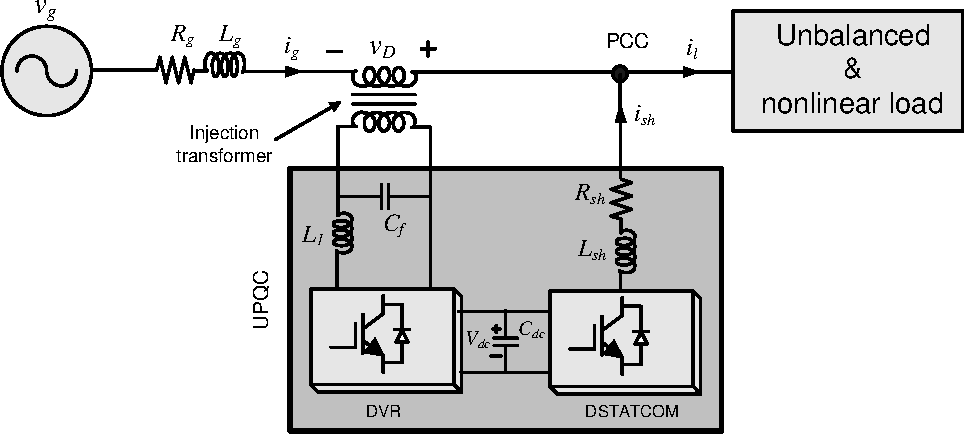
\includegraphics[scale=0.88]{figures/Chapter_1_2/fig2p2}
	\caption{Single-line diagram of UPQC-R configuration}
	\label{fig2.2}
\end{figure}


\begin{figure}[ht]
	\centering
	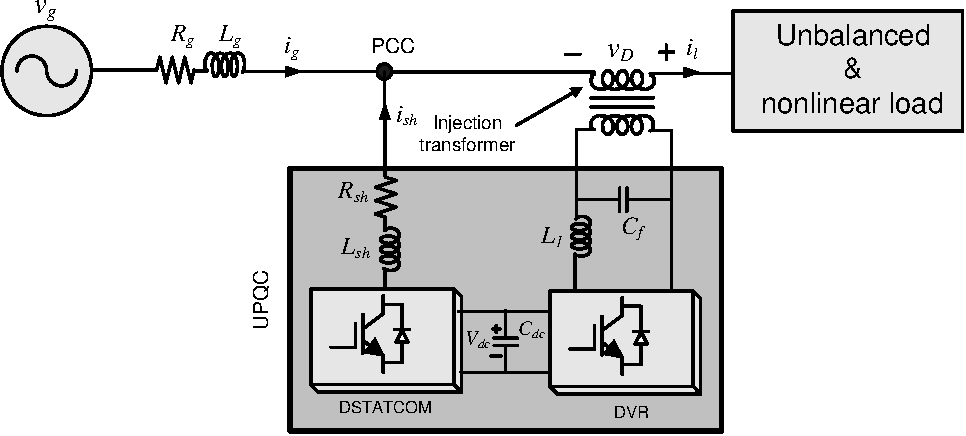
\includegraphics[scale=0.88]{figures/Chapter_1_2/fig2p3}
	\caption{Single-line diagram of UPQC-L configuration}
	\label{fig2.3}
\end{figure}

The flow of zero sequence current in the neutral wire is quite common in the 3P4W DG system. The VSI interfaced with such 3P4W systems must provide a path for the flow of zero-sequence current. Thus, the four-leg VSI topology is used for shunt compensator. The converter topology of series compensator can be either three-leg VSI or four-leg VSI based on the UPQC configuration. In \cite{ghosh2002power,6095377}, two possible configurations of UPQC at the PCC have been discussed. One is the right shunt UPQC (UPQC-R), in which the shunt compensator is connected to the load side and the series compensator to the supply side, as shown in Fig. \ref{fig2.2}. The second one is the left shunt UPQC (UPQC-L), in which the shunt compensator is connected to the supply side and the series compensator to the load side, as shown in Fig. \ref{fig2.3}. In the UPQC-R configuration, the shunt VSI carries all the zero-sequence load current, while the series VSI does not carry any zero-sequence load current, making it possible to use a three-leg VSI for the series compensator. In contrast, there is a possibility of zero sequence current flow through series VSI in UPQC-L configuration and hence four-leg VSI has to be used in UPQC-L. Thus, UPQC-R requires less number of semiconductor switches compared to UPQC-L.      

%The main purpose of a UPQC is to compensate for supply voltage flicker/imbalance, reactive power, negative-sequence current and harmonics.
%In other words, the UPQC has the capability of correcting the voltage and current at the point of installation on power distribution systems or industrial power systems. The UPQC, therefore, is expected to be one of the most powerful solutions to all the power quality issues. 

%Figure \ref{fig2.1} shows the power circuit of the neutral clamped VSI topology based UPQC. In this figure, $v_{sa}$, $v_{sb}$ and $v_{sc}$ are source voltages of phases $a$, $b$ and $c$, respectively. Similarly, $v_{ta}$, $v_{tb}$ and $v_{tc}$ are the terminal voltages . The voltages $v_{dvra}$, $v_{dvrb}$ and $v_{dvrc}$ are the voltage injected by the series active filter. The source currents in three phase are represented by $i_{sa}$, $i_{sb}$ and $i_{sc}$, load currents are represented by $i_{la}$, $i_{lb}$ and $i_{lc}$. The shunt active filter currents are denoted by $i_{fa}$, $i_{fb}$, $i_{fc}$ and  $i_{ln}$ represents the  current in the neutral leg. $L_s$ and $R_s$ represent the feeder inductance and resistance, respectively. The interfacing inductance and resistance of the shunt active filter are represented by $L_f$ and $R_f$ respectively. The shunt filter capacitor is represented by $C_{sh}$. The interfacing inductance and filter capacitor of the series active filter are represented by $L_{se}$ and $C_{se}$ respectively.  The load constituted of both linear and nonlinear loads  as shown in this figure. The DC-link capacitors and voltages across them are represented by $C_{dc1}$ = $C_{dc2}$ = $C_{dc}$ and  $V_{dc1}$ =  $V_{dc2}$ =  $V_{dc}$, respectively.

%\begin{sidewaysfigure}[]
%	\centering
%		\includegraphics[scale=1.354]{figures/Chapter_1_2/fig2p1}
%	
%\caption{Power circuit of three phase UPQC.}
%
%		\label{fig2.1}
%\end{sidewaysfigure}

\section{DUAL-OUTPUT CONVERTER} \label{2.Section_DOC}

Currently, approximately 30\% of all the electric power generated uses power electronics somewhere between the point of generation and distribution. Some analysts project that 80\% of the energy will flow through power electronics in the near future, but that would require cost reductions in power electronics and power conversion systems. In line with this, recent research has been focused on high power density converter topologies. The high power density can be achieved by using wide-band semiconductor switches and/or reduced number of switches in a converter topology. This thesis focuses on the reduced switch count converter topologies for UPQC system. One of them is the dual-output converter (DOC). It is also called as nine-switch converter (NSC) in 3P3W systems as it contains only nine semiconductor switches. The NSC was introduced in \cite{4348103} for the motor drive applications. In this section, a brief overview of the dual-output converter is presented including its
topology characteristics and modes of operation.
\begin{figure}[ht]
	\centering
	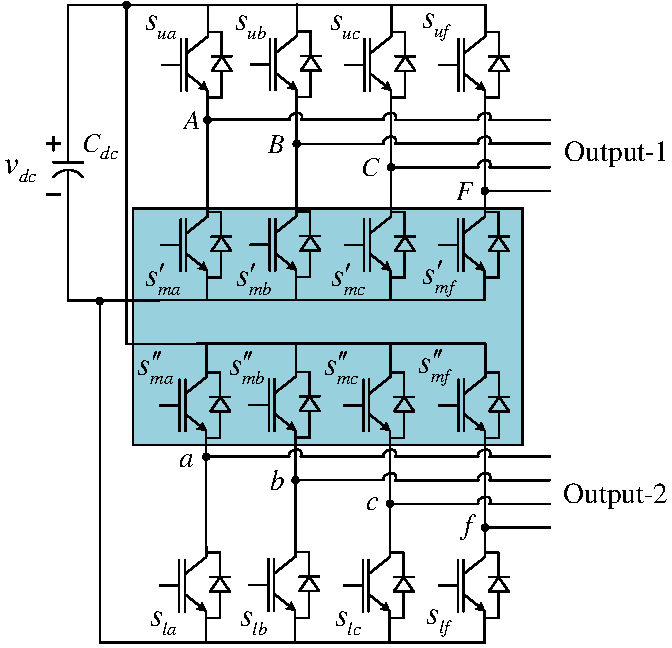
\includegraphics[scale=0.88]{figures/Chapter_1_2/BTB}
	\caption{Back-to-back (BTB) converter configuration}
	\label{2.BTB}
\end{figure}

The DOC is similar to conventional back-to-back (BTB) configuration in which bottom switches of one converter and top switches of other converter combine to form middle switches of DOC. As a result of this new arrangement, the total number of switches are reduced from sixteen to twelve with respect to its counterpart. Moreover, both the BTB topology and the DOC are able to generate and control two sets of three-phase signals with different amplitude, frequency and phase shift. The DOC experiences its own structural limitations, however it is usually the case for converters with a reduced number of semiconductor switching devices. The structure of BTB topology and DOC are shown in Figs.\,\ref{2.BTB} and \ref{2.DOC}, respectively. The DOC is actually built with a single capacitor at DC-link. However, the split-capacitor based DC-bus is shown in Fig.\,\ref{2.DOC} to understand the switching states of DOC described below. 
\begin{figure}[ht]
	\centering
		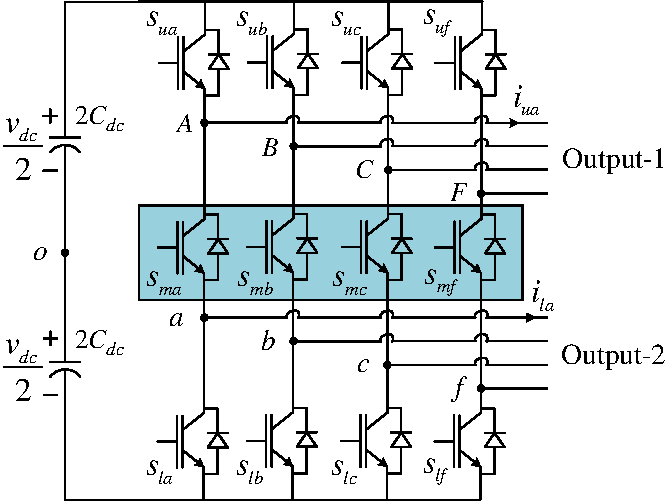
\includegraphics[scale=0.88]{figures/Chapter_1_2/DOC}
	\caption{Dual-output converter (DOC) configuration}
	\label{2.DOC}
\end{figure}
\begin{table}[h]
	\centering
	\caption{Possible switching states of dual output converter}
	%\resizebox{\linewidth}{!}{ \footnotesize
	\begin{tabu}{cccccc}
		\tabucline[1pt]{-}           % Top thick line
		&  &  & \multicolumn{3}{c}{\footnotesize \textbf{Direction}}  \\
		\cline{4-6}
		\multirow{-2}{*}{\footnotesize$\mathbf{S_{ua}~S_{ma}~S_{la}}$}  &  \multirow{-2}{*}{\footnotesize \boldmath{$v_{Ao}$}}    & \multirow{-2}{*}{\footnotesize \boldmath{$v_{ao}$}}  & \footnotesize$\mathbf{i_{ua}}$ & \footnotesize$\mathbf{i_{la}}$ & \footnotesize$\mathbf{i_{ua} + i_{la} }$\\
		\tabucline[1pt]{-}
		%\hline
		
		\rowcolor{lightgray} \scriptsize 0\hspace{0.5cm}1\hspace{0.5cm}1 & \scriptsize \si{-} & \scriptsize \si{-} & \footnotesize A & \footnotesize A & \footnotesize A  \\
		%\hline
		
		\rowcolor{lightgray} \scriptsize 1\hspace{0.5cm}1\hspace{0.5cm}0 & \scriptsize \si{+} & \scriptsize \si{+} & \footnotesize A & \footnotesize A & \footnotesize A \\
		%\hline
		
		\rowcolor{lightgray} \scriptsize 1\hspace{0.5cm}0\hspace{0.5cm}1 & \scriptsize \si{+} & \scriptsize \si{-} &  \footnotesize A & \footnotesize A &  \footnotesize A \\
		\hline
		
		\multirow{2}{*}{\textcolor{black}{\scriptsize 0\hspace{0.5cm}1\hspace{0.5cm}0}} & \textcolor{black}{\scriptsize \si{+}} & \textcolor{black}{\scriptsize \si{+}} & A & A & N \\ %\cline{2-6}
		&  \textcolor{black}{\scriptsize \si{-}} & \textcolor{black}{\scriptsize \si{-}} & A & A & P \\ 
		\hline
		
		& \textcolor{black}{\scriptsize \si{+}} & \textcolor{black}{\scriptsize \si{+}} & A & N & N \\ %\cline{2-6}
		\textcolor{black}{\scriptsize 0\hspace{0.5cm}0\hspace{0.5cm}0} & \textcolor{black}{\scriptsize \si{-}} & \textcolor{black}{\scriptsize \si{-}} & P & A & P\\ %\cline{2-6}
		&           \textcolor{black}{\scriptsize \si{+}} & \textcolor{black}{\scriptsize \si{-}} & N & P & A \\ 
		\hline
		
		\multirow{2}{*}{\textcolor{black}{\scriptsize 0\hspace{0.5cm}0\hspace{0.5cm}1}} & \textcolor{black}{\scriptsize \si{-}} & \textcolor{black}{\scriptsize \si{-}} & P & A & A \\ %\cline{2-6}
		&  \textcolor{black}{\scriptsize \si{+}} & \textcolor{black}{\scriptsize \si{-}} & N & A & A \\ 
		\hline
		
		\multirow{2}{*}{\textcolor{black}{\scriptsize 1\hspace{0.5cm}0\hspace{0.5cm}0}} & \textcolor{black}{\scriptsize \si{+}} & \textcolor{black}{\scriptsize \si{+}} & A & N & A \\ %\cline{2-6}
		&  \textcolor{black}{\scriptsize \si{+}} & \textcolor{black}{\scriptsize \si{-}} & A & P & A \\ 
		\hline
		
		& \textcolor{black}{\scriptsize \si{+}} & \textcolor{black}{\scriptsize \si{+}} & P & P & P \\ %\cline{2-6}
		\textcolor{black}{\scriptsize 1\hspace{0.5cm}1\hspace{0.5cm}1} & \textcolor{black}{\scriptsize \si{-}} & \textcolor{black}{\scriptsize \si{-}} & N & A & A\\ %\cline{2-6}
		&           \textcolor{black}{\scriptsize \si{+}} & \textcolor{black}{\scriptsize \si{-}} & P & N & A \\ 
		\tabucline[1pt]{-}
		
		\multicolumn{6}{c}{\footnotesize `\si{+}'~:~$\frac{V_{dc}}{2};$ \hspace{0.1cm} `\si{-}'~:~$\frac{-V_{dc}}{2};$ \hspace{0.1cm} P~:~ Positive; \hspace{0.1cm} N~:~ Negative; \hspace{0.1cm} A~:~ Any }  
	\end{tabu} %}
	\label{Table2.1} \vspace*{-0.4cm}
\end{table}
\begin{figure}[h]
	\centering
	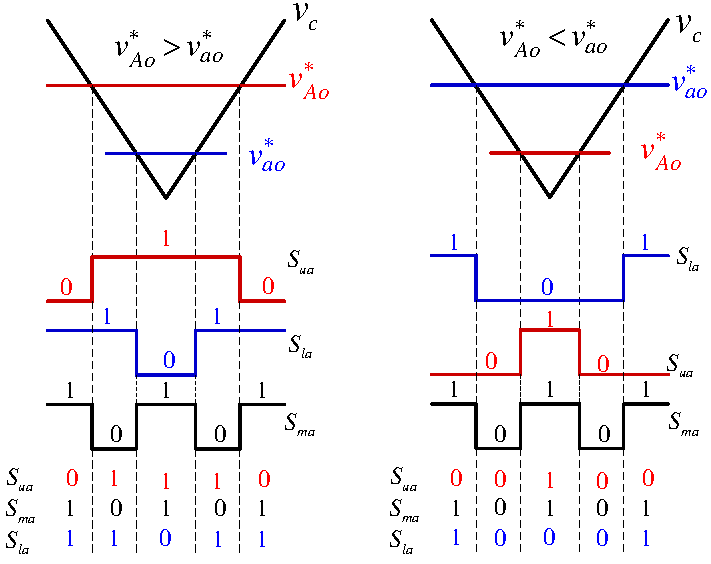
\includegraphics[scale=0.88]{figures/Chapter_1_2/Switching_Diagram_NSC}
	\caption{Switching diagram of SPWM for DOC}
	\label{2.switchingSPWM}
\end{figure}


Consider phase - \textit{a} leg of the converter shown in Fig.\,\ref{2.DOC}. There are eight possible switching states as it has three switches in a leg. In Table\,\ref{Table2.1}, the pole voltages ($v_{Ao}$, $v_{ao}$) are tabulated against each switching state for all possible directions of the currents. Among eight states, only the first three states listed in Table\,\ref{Table2.1} are having a unique pole voltage irrespective of current directions and thus these three states are valid. From these valid states, it is observed that the state of middle switch can be generated using either logical NAND or XOR operation of upper and lower switch states.

In sinusoidal pulsewidth modulation (SPWM), the elimination of invalid switching states is achieved by introducing offsets to the modulating signals of both the upper output (output-1) and lower output (output-2). This adjustment ensures that the upper signal is consistently higher than the lower signal, preventing the occurrence of undesirable switching states \cite{4348103} as shown in Fig.\,\ref{2.switchingSPWM}. The state of upper switch ($S_{ua}$) is determined by comparing the upper output modulating signal ($v^{*}_{Ao}$) with the carrier signal ($v_c$). If $v^{*}_{Ao} > v_{c}$, $S_{ua}$ is set to high, indicating that the top switch should be turned on. Similarly, the state of bottom switch ($S_{la}$) is determined by comparing the lower output modulating signal ($v^{*}_{ao}$) with the carrier signal ($v_c$). If $v^{*}_{ao} < v_{c}$, $S_{la}$ is set to high, indicating that the bottom switch should be turned on. The state of the middle switch ($S_{ma}$) is determined by applying a logical XOR operation to the states of the lower and upper switches. By using XOR, the invalid switching state $000$ is observed when $v^{*}_{Ao} < v^{*}_{ao}$. If the logical XOR was replaced with a NAND operation, then the invalid switching state $010$ would be noticed for $v^{*}_{Ao} < v^{*}_{ao}$. According to Table\,\ref{Table2.1}, the state $000$ has three possible voltage outputs \{$(+,+),(-,-),(+,-)$\}, whereas the state $010$ has only two voltage possibilities \{$(+,+),(-,-)$\}. Therefore, NAND operation is preferred to determine the state of the middle switch as it simplifies converter control by having the state with least voltage output possibilities.
\begin{figure}[ht]
	\centering	
	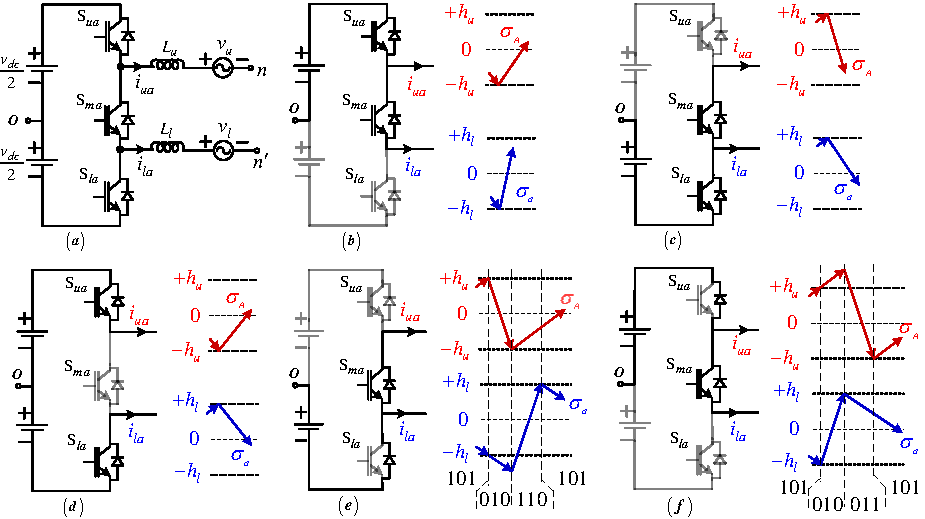
\includegraphics[scale=1]{figures/Chapter_1_2/Direct_modul}
	\caption{(a) 1-$\phi$ half bridge DOC; switching states: (b) 110, ~~(c) 011, ~~(d) 101, ~~ (e) 010 resembles as 011 due to net positive current, ~~ (f) 010 resembles as 110 due to net negative current }
	\label{2.direct_modul}
\end{figure}


In sliding mode (SM) PWM, the states of the upper and lower switches are determined based on the position of structured sliding surface trajectories. Let's consider a single-phase DOC designed for current control of two independent loads, as shown in Fig.\,\ref{2.direct_modul}(a) \cite{6563653}. The filter inductance, load voltage and load neutral of upper output are denoted as $L_u, \, v_u$, and $n$, respectively. Similarly, the filter inductance, load voltage and load neutral of lower output are denoted as $L_l, \, v_l$, and $n^{\prime}$, respectively. The sliding surface is structured as $\sigma_{A} = i_{ua} - i^{*}_{ua} = 0$ for the upper output and $\sigma_{a} = i_{la} - i^{*}_{la} = 0$ for the lower output. Here, $i_{ua}$ and $i^{*}_{ua}$ represent the actual and reference currents of the upper output, respectively, while $i_{la}$ and $i^{*}_{la}$ denote the actual and reference currents of the lower output, respectively. All these currents are associated with phase-$a$ of their respective outputs. The switching logics are selected in a way that the sliding variable should be maintained at zero. To achieve this, the top switch is turned `OFF' ($S_{ua}=0$) when the trajectory of upper sliding variable ($\sigma_{A}$) reaches its upper hysteresis band ($+h_{u}$). Conversely, when the trajectory of $\sigma_{A}$ reaches the lower band ($-h_{u}$), the top switch is turned `ON' ($S_{ua}=1$). Similarly, when the trajectory of the lower sliding variable ($\sigma_{a}$) reaches its upper band ($+h_{l}$), the bottom switch is turned `ON' ($S_{la}=1$). Conversely, when the trajectory of $\sigma_{a}$ reaches the lower band ($-h_{l}$), the bottom switch is turned `OFF' ($S_{la}=0$). 

Let's analyze the operation of SM-PWM using four different instants, as depicted in Fig.\,\ref{2.direct_modul}(b)-(f). The first instant is considered when both sliding variables reach their lower hysteresis bands, as shown in Fig.\,\ref{2.direct_modul}(b). According to the discussed switching logics, the switching state $110$ is applied. In this state, both pole voltages ($v_{Ao}$ and $v_{ao}$) are set to $+\frac{v_{dc}}{2}$, causing the sliding variables to increase. This modulation helps to keep the sliding variables within their respective bands. Similar scenarios can be observed when $\sigma_{A}$ and $\sigma_{a}$ reach their upper hysteresis bands, as shown in Fig.\,\ref{2.direct_modul}(c), or when $\sigma_{A}$ reaches its lower band and $\sigma_{a}$ reaches its upper band, as shown in Fig.\,\ref{2.direct_modul}(d). According to the switching logics, the switching state $011$ and $101$ are applied, respectively.

In the last instant, $\sigma_{A}$ reaches its upper band and $\sigma_{a}$ reaches its lower band, as shown in Fig.\,\ref{2.direct_modul}(e)-(f). According to the discussed switching logics, the invalid switching state $010$ is applied. When the net load current ($i_{ua} + i_{la}$) is positive, the freewheeling diode of bottom switch conducts and it resembles the $011$ switching state, as shown in Fig.\,\ref{2.direct_modul}(e). In this state, both pole voltages are set to $-\frac{v_{dc}}{2}$, causing the sliding variables to decrease. As a result, $\sigma_{A}$ stays within its band but $\sigma_{a}$ deviates from its lower band and continues to deviate until $\sigma_{A}$ reaches its lower band. A similar case is observed when the net load current is negative. In this situation, the freewheeling diode of top switch conducts and it resembles $110$ switching state, as shown in Fig.\,\ref{2.direct_modul}(f). Both pole voltages are set to $+\frac{v_{dc}}{2}$, causing the sliding variables to increase. Consequently, $\sigma_{a}$ stays within its band but $\sigma_{A}$ deviates from its upper band and continues to deviate until $\sigma_{a}$ reaches its upper band. In both the cases, to minimize the magnitude of sliding variables deviating from their bands, it is necessary to satisfy the below condition:
\begin{equation}
\dot{\sigma}_{a} > \dot{\sigma}_{A}. 
\label{eqn2.1(1)}
\end{equation}       
Over a switching period, the reference currents are assumed to remain constant, considering a switching frequency that is much higher than the fundamental frequency. Therefore \eqref{eqn2.1(1)} can be rewritten as follows:
\begin{equation}
\begin{split}
\dot{i}_{la} - \dot{i}^{*}_{la} &> \dot{i}_{ua} - \dot{i}^{*}_{ua}, \\
\Rightarrow \hspace{2.3cm} \dot{i}_{la} &> \dot{i}_{ua}, \\
\Rightarrow \hspace{0.15cm} \frac{v_{ao} - v_{l} - v_{n^{\prime}o}}{L_l}  &> \frac{v_{Ao} - v_{u} - v_{no}}{L_u}.
\end{split}
\label{eqn2.1(2)}
\end{equation}
The pole voltages ($v_{Ao}$ and $v_{ao}$) are equal in both cases of the last instant. Assuming equal filter inductances, \eqref{eqn2.1(2)} can be updated as follows:
\begin{equation}
\begin{split}
v_{u} + v_{no} &> v_{l} + v_{n^{\prime}o}, \\
\Rightarrow v^{*}_{Ao} &> v^{*}_{ao}. 
\end{split}
\label{eqn2.1(3)}
\end{equation}
 
It says that by consistently maintaining upper output pole voltage higher than the lower output pole voltage, the sliding variables can converge to their hysteresis bands within a finite time, even if the deviations occur. This condition is similar to that of SPWM, where it is necessary to avoid the invalid switching state. However, achieving this condition in SMPWM is not as straightforward as in SPWM. In SMPWM, it can be realized by using the external control degree of freedoms, i.e., common mode voltages $v_{no}$ and $v_{n^{\prime}o}$. These additional control parameters provide the means to ensure that the upper output pole voltage remains consistently higher than the lower output pole voltage, facilitating the convergence of the sliding variables to their respective hysteresis bands.


\section{DUAL-OUTPUT CONVERTER BASED UPQC } \label{2.DOC_UPQC}

The dual-output converter has been widely used in various applications, as reported in \cite{4342442, 4417438, 5446393, 5754572, 5445017, 6563653, 9547678}. However, many of these applications involve replacing the back-to-back converter with two shunt VSCs, which does not fully utilize the potential of this new topology. This issue was discussed in \cite{5542338} and \cite{5713844}. As a solution, it has been proposed to use the dual-output converter for replacing back-to-back converter in "series-shunt" systems such as UPQC-L. This design concept is illustrated in Fig.\,\ref{2.NS-UPQC} for 3P3W distribution system.
\begin{sidewaysfigure}[]
	\centering	
	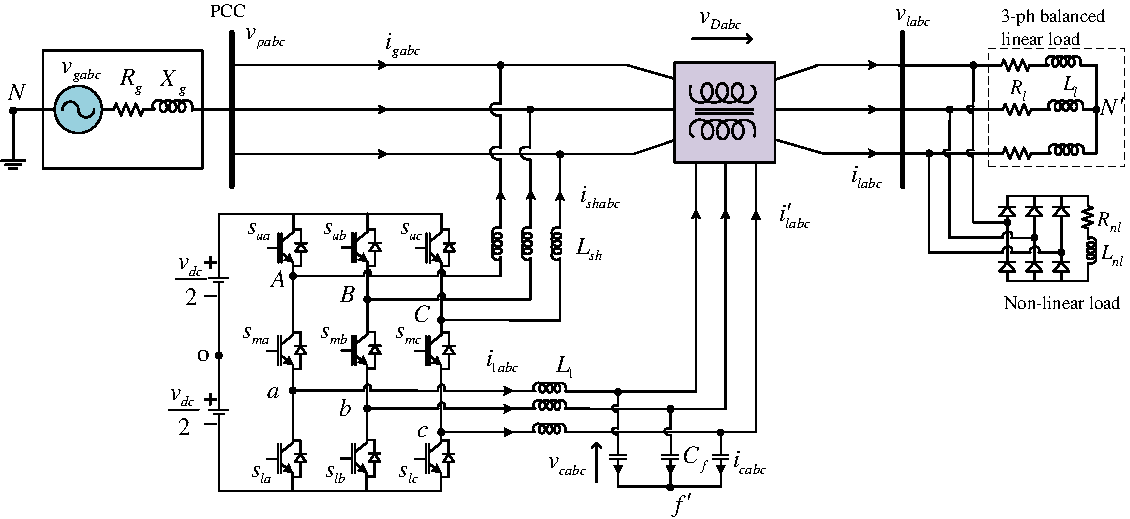
\includegraphics[scale=1]{figures/Chapter_6/Mine/NS_UPQC_L}
	\caption{Nine-switch UPQC}
	\label{2.NS-UPQC}
\end{sidewaysfigure}

Fig.\,\ref{2.NS-UPQC} depicts the nine-switch UPQC configuration with the left shunt, where a single DC source is replaced with split-source for a better understanding of converter dynamics. The shunt and series passive filters were represented by $L_{sh}$ and parallel $L_{1} C_{f}$, respectively. The switching mechanism of the nine-switch converter was explained in Section \ref{2.Section_DOC}. The shunt and series terminals function similarly to those of a conventional UPQC, as mentioned in Section \ref{2.Section_UPQC}. However replacing BTB topology with the NSC, novel operating principles of the shunt and series terminals were introduced for normal and 20\% sag conditions in \cite{5713844}.

The division of carrier range between the shunt and series terminals during normal operation and voltage sag conditions, as discussed in \cite{5713844}, is depicted in Fig.\,\ref{2.carrier}. In this scenario, the placement of upper and lower modulating references are for the shunt and series terminals, respectively. Under the normal voltage operating condition, the maximum existence of harmonics in supply voltage is about 5\%. Thus, the carrier range is divided with a much wider vertical range $h_1$ for controlling the shunt terminal and a narrower $h_2$ for controlling the series terminal to compensate 5\% harmonics.   
\begin{figure}[ht]
	\centering	
	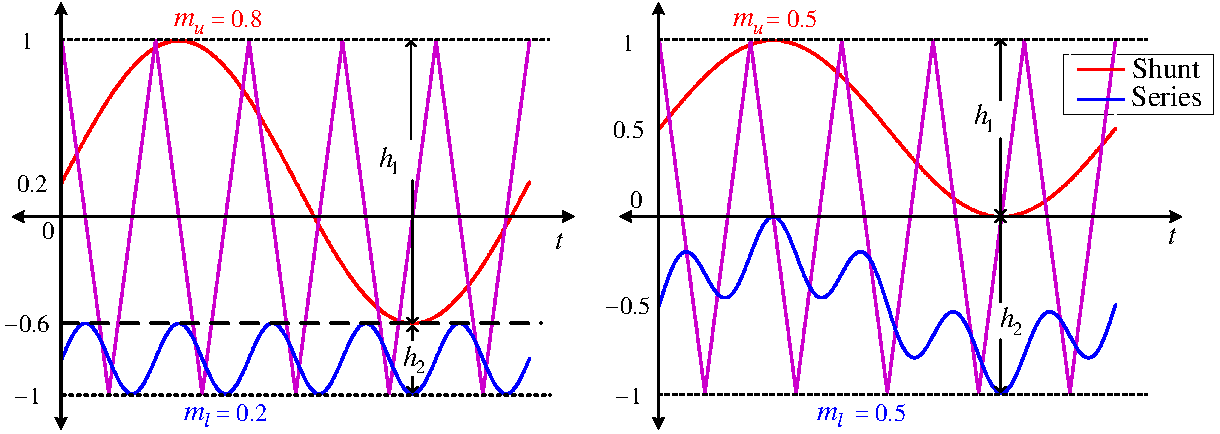
\includegraphics[scale=0.7]{figures/Chapter_1_2/fig3}
	\caption{Modulating references during normal (left) and voltage sag (right) modes}
	\label{2.carrier}
\end{figure}

Under voltage sag condition, the shunt terminal at the point of common coupling (PCC) experiences a reduced voltage. This reduction in voltage requires a corresponding reduction in $h_1$, thereby freeing up more carrier space for the series reference to vary within, ensuring that interference between the shunt and series references is avoided. 

If this carrier division approach is applied to UPQC-R configuration, then the carrier range of shunt terminal is fixed at [-1,1] assuming series compensator functions normally and its terminal voltage is always at 1 pu. During severe sag conditions, such as a sag of 1 pu, the carrier range of series terminal is also [-1,1]. As a result, the DC-link voltage required for the UPQC-R configuration is twice as high as that required for the UPQC-L configuration. When applying the same approach to the UPQC-L configuration for compensating voltage swells, the shunt reference overlaps with the series reference at normal DC-link voltage. Consequently, a higher DC-link voltage is required to ensure that the references do not interfere with each other. 

Moreover, the appropriate control and modulation schemes developed for the nine-switch UPQC are presented in \cite{5713844}. The $120^{\circ}$-\,discontinuous modulation technique is implemented for both the shunt and series terminals, and the control schemes with linear controllers are described for both terminals separately according to their main functions. The synchronous reference frame (SRF) theory was used for the generation of reference currents and voltages.

The design of the shunt terminal controller focuses on load current harmonic compensation, reactive power injection, and maintaining the DC-link voltage at the desired level. The sensed load currents are first transformed into $d$ and $q$ components by Park's transformation. Next, the harmonic components of load currents are obtained by passing the d-axis load current ($i_d$) through high-pass filter (HPF). This filtered signal of d-axis harmonics is added with a d-axis control reference of a DC-link proportional-integral (PI) regulator. The regulator compensates the losses and maintains the DC-link voltage constant. The $q$ component of load current ($i_q$) contributes to the load reactive power compensation. Finally, the generated $d$ and $q$ reference components are transformed back to the abc natural frame, and the error between the shunt reference and measured currents is sent to a proportional-resonant (PR) controller that generates switching pulses. A block diagram of this control technique is shown in Fig.\,\ref{2.Shunt_control}.
\begin{figure}[ht]
	\centering	
	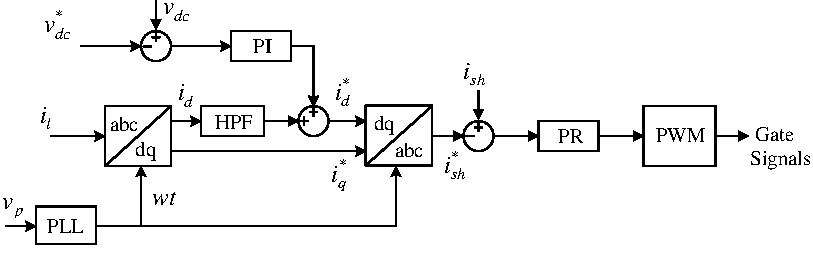
\includegraphics[scale=1]{figures/Chapter_1_2/fig4}
	\caption{Conventional control circuit of shunt compensator \cite{5713844}}
	\label{2.Shunt_control}
\end{figure}

The control scheme for the series terminal is depicted in Fig.\,\ref{2.Series_control}, using a multi-loop control approach. Its primary functions are to compensate voltage harmonics in the utility grid or DG system and to maintain load voltage at the desired level during grid voltage variations. Selective harmonic compensation was implemented in the subsystem for voltage harmonic compensation, following the method described in \cite{1185456}. The second part of the series terminal control system, i.e., the feed-forward PI regulator was designed with two degrees of freedom for detecting sags and accounting for voltage drops across the inductive components, including series transformers and inductors.
\begin{figure}[ht]
	\centering	
	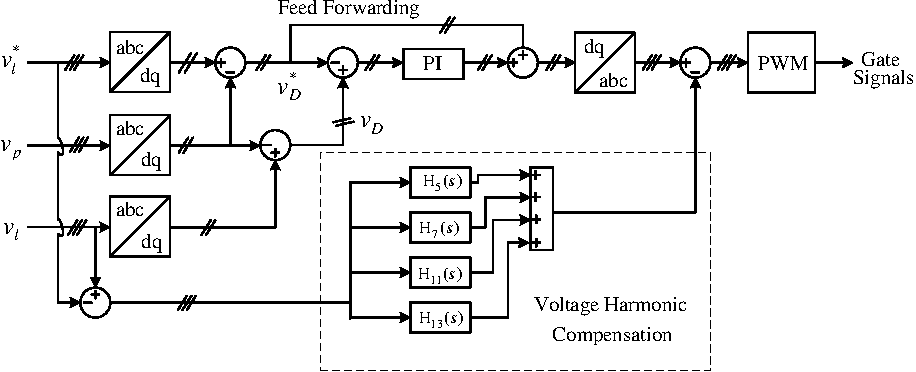
\includegraphics[scale=0.95]{figures/Chapter_1_2/fig5}
	\caption{Conventional control circuit of series compensator \cite{5713844}}
	\label{2.Series_control}
\end{figure}

The shunt and series terminal controllers were designed using linear control methods, which can cause some issues. Firstly, the reference waveforms for both terminals were generated using the SRF theory with the complicated Park's transformation. Secondly, to mitigate current/voltage harmonics, the PR controller needs to have cascaded resonant blocks that must be tuned for each desired harmonic frequency, making the controller complex and able to mitigate only the most prominent harmonics in the frequency spectrum \cite{IEE-EPA}. Thirdly, the feed-forward path to compensate voltage drops across reactive elements requires the series terminal controller to be implemented in a multi-loop configuration. Also, due to the poor low-order harmonic mitigation capability of the PI controller, multiple resonant regulators were placed, resulting in slight transient sluggishness to maintain stability \cite{5713844}. As the system order increases, tuning of the PI and PR controllers becomes more complicated.

\section{CONTROL OF UPQC}
Generating reference quantities and realizing them using voltage source inverters (VSIs) are two crucial tasks in the control of any active power filter. This section presents various control algorithms for generating reference quantities and techniques for controlling the switching of VSIs. 
\vspace*{-1.5cm}
\subsection {Generation of Reference Quantities for DSTATCOM}

The choice of a control strategy for generating reference quantities significantly impacts the compensation performance of an active filter. In the literature, several power theories have been presented for reference generation \cite{otto1978principles,gyugyi1979reactive,41770,akagi1986control,akagi1984instantaneous,akagi1983generalized,peng1996generalized,peng1998harmonic,ghosh1998new,847283,ghosh2000use,Benhabib2005353,chen1993reactive, 4283506}. Among these, the instantaneous reactive power theory \cite{akagi1986control,akagi1984instantaneous,akagi1983generalized}, generalized instantaneous reactive power theory \cite{peng1996generalized}, synchronous reference theory \cite{Benhabib2005353}, and instantaneous symmetrical components theory \cite{ghosh1998new,847283,ghosh2000use} are commonly utilized. In this section, a concise overview of these theories are provided.
\vspace*{-1.5cm}
\subsubsection{Instantaneous Reactive Power Theory \cite{Mahesh_Mishra}} 
\vspace*{-0.5cm}
"The Instantaneous Reactive Power Theory was initially proposed by Akagi H., Kanazawa Y., and Nabae A. in 1983-84 \cite{akagi1984instantaneous}. The primary objective of this theory is to establish a mathematical framework for calculating instantaneous reactive power, enabling the compensation of reactive power not only in steady-state but also during transient conditions. This theory is commonly employed to determine the reference current for a shunt active filter. It utilizes the instantaneous values of voltages and currents to derive the compensating quantities. To facilitate this process, the $abc$ phase voltages and currents are transformed to the stationary $\alpha$ - $\beta$ axis using the Clarke transformation, which is depicted in Fig. \ref{fig2.4a}.
\begin{figure}[ht]
	\centering
		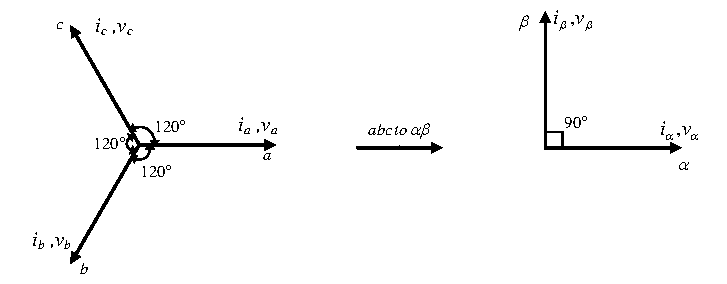
\includegraphics[scale=1.1]{figures/Chapter_1_2/fig2p4a}
	\caption{\textit{abc} to $\alpha\beta$ transformation}
	\label{fig2.4a}
\end{figure}

The instantaneous \textit{abc} phase voltages are transformed into $\alpha$-$\beta$-\textit{0} coordinates to include the zero sequence components, as given below.
\begin{equation}
\begin{bmatrix} v_0 \\ v_\alpha \\ v_\beta
\end{bmatrix}= \sqrt{\frac{2}{3}}\begin{bmatrix} \frac{1}{\sqrt{2}}& \frac{1}{\sqrt{2}} & \frac{1}{\sqrt{2}} \\ 1 & -\frac{1}{2} & -\frac{1}{2} \\
0 & \frac{\sqrt{3}}{2} & -\frac{\sqrt{3}}{2}
\end{bmatrix} \begin{bmatrix} v_a  \\
v_b \\ v_c
\end{bmatrix} ; 
\begin{bmatrix} i_0 \\ i_\alpha \\ i_\beta
\end{bmatrix}= \sqrt{\frac{2}{3}}\begin{bmatrix} \frac{1}{\sqrt{2}}& \frac{1}{\sqrt{2}} & \frac{1}{\sqrt{2}} \\ 1 & -\frac{1}{2} & -\frac{1}{2} \\
0 & \frac{\sqrt{3}}{2} & -\frac{\sqrt{3}}{2}
\end{bmatrix} \begin{bmatrix} i_a  \\
i_b \\ i_c
\end{bmatrix}
\label{eqn2.1}
\end{equation}
The instantaneous real power is defined as the product of the instantaneous voltage and the instantaneous current, both aligned along the same axis. \vspace*{-0.5cm}
\begin{equation}
p=v_\alpha i_\alpha + v_\beta i_\beta
\label{eqn2.2}
\end{equation} %\vspace*{-1cm}
In \textit{abc} coordinates it is given by, \vspace*{-0.5cm} 
\begin{equation*}
p=v_a i_a + v_b i_b + v_c i_c.
\end{equation*}
The instantaneous reactive power is defined as the cross product of the instantaneous voltage along one axis and the instantaneous current along its quadrature axis. 
\begin{equation}
q  =  \stackrel{\rightarrow}{v}_\alpha \times \stackrel{\rightarrow}{i}_\beta + \stackrel{\rightarrow}{v}_\beta \times \stackrel{\rightarrow}{i}_\alpha 
\label{eqn2.3}
\end{equation} \vspace*{-1cm}
\begin{equation}
q  =   v_\alpha i_\beta - v_\beta i_\alpha 
\label{eqn2.4}
\end{equation} \vspace*{1cm}
Using (\ref{eqn2.1}) and (\ref{eqn2.3}), the expression for the same in \textit{abc} coordinates is given below. \vspace*{-1cm}
\begin{equation}
q= -\frac{1}{\sqrt{3}}[(v_a - v_b)i_c + (v_b - v_c)i_a + (v_c - v_a)i_b]
\label{eqn2.5}
\end{equation} \vspace*{-1cm}
\begin{equation}
q= -\frac{1}{\sqrt{3}}[v_{ab}i_c + v_{bc}i_a + v_{ca}i_b]
\label{eqn2.6}
\end{equation}
The instantaneous zero sequence power is defined as $p_o$ = $v_0$$i_0$.
The instantaneous powers in $\alpha\beta 0$- coordinates can be represented in the following matrix form.
\begin{equation}
\begin{bmatrix} p_0 \\p \\ q
\end{bmatrix}= \begin{bmatrix} v_0 &  0 & 0 \\ 0 & v_\alpha & v_\beta \\ 0 & -v_\beta  & v_\alpha
\end{bmatrix} \begin{bmatrix} i_0 \\i_\alpha  \\
i_\beta
\end{bmatrix}
\label{eqn2.7}
\end{equation}
It can be rearranged in the following form.
\begin{equation}
\begin{aligned}
\begin{bmatrix} i_0 \\i_\alpha  \\
i_\beta
\end{bmatrix} &= {\begin{bmatrix} v_0 &  0 & 0 \\ 0 & v_\alpha & v_\beta \\ 0 & -v_\beta  & v_\alpha
\end{bmatrix}}^{-1} \begin{bmatrix} p_0 \\p \\ q
\end{bmatrix} \\ &= \frac{1}{v_0 ({v_\alpha^2 + v_\beta^2})}  \begin{bmatrix} {v_\alpha^2 + v_\beta^2} & 0 & 0 \\ 0 & v_0 v_\alpha & -v_0 v_\beta \\ 0 & v_0 v_\beta & v_0 v_\alpha
\end{bmatrix} \begin{bmatrix} p_0 \\p \\ q
\end{bmatrix} \\ &= \begin{bmatrix} i_{0 p} \\ 0 \\ 0
\end{bmatrix} + \begin{bmatrix} 0 \\ i_{\alpha p} \\ i_{\beta p}
\end{bmatrix} +\begin{bmatrix} 0 \\ i_{\alpha q} \\ i_{\beta q} 
\end{bmatrix}
\label{eqn2.8}
\end{aligned}
\end{equation}
The various terms in the above equation are defined as follows.

Zero sequence current, $i_{0p} = p_0/v_0$,

$\alpha$- axis instantaneous active current, $i_{\alpha p}$ = ${v_\alpha} p/({v_\alpha^2 + v_\beta^2})$,

$\alpha$- axis instantaneous reactive current, $i_{\alpha q}$ = $-{v_\beta} q/({v_\alpha^2 + v_\beta^2})$,

$\beta$- axis instantaneous active current, $i_{\beta p}$ = ${v_\beta} p/({v_\alpha^2 + v_\beta^2})$,

$\beta$- axis instantaneous reactive current, $i_{\beta q}$ = ${v_\alpha} q/({v_\alpha^2 + v_\beta^2})$.

Using (\ref{eqn2.8}), the components of the filter current in terms of its powers and voltages can be expressed as shown below.
\begin{equation}
\begin{bmatrix} i_{f0} \\i_{f \alpha}  \\
i_{f \beta}
\end{bmatrix} = \frac{1}{v_0 ({v_\alpha^2 + v_\beta^2})}  \begin{bmatrix} {v_\alpha^2 + v_\beta^2} & 0 & 0 \\ 0 & v_0 v_\alpha & -v_0 v_\beta \\ 0 & v_0 v_\beta & v_0 v_\alpha
\end{bmatrix} \begin{bmatrix} p_{f0} \\p_f \\ q_f
\end{bmatrix}
\label{eqn2.12}
\end{equation}
Where, $i_{f0}, \, i_{f \alpha}$ and $i_{f \beta}$ represent the reference filter currents, while $p_{f0}, \, p_f$ and $q_f$ correspond to the powers that need to be compensated. The instantaneous real and reactive powers of the load are divided as follows.

$p_L=\bar{p}_L + \tilde{p}_L + p_{L0}$ and $q_L=\bar{q}_L + \tilde{q}_L$, where $\bar{p}_L$ and $\tilde{p}_L$ are the DC and AC components of the instantaneous real power, $p_{L0}$ is the zero-sequence power and  $\bar{q}_L$ and $\tilde{q}_L$ are the DC and AC components of the instantaneous reactive power. Here the subscript `L' represents load in the system.

By selecting $p_f$ = $\tilde{p}_L$, $p_{f0} = p_{L0}$ and $q_f$ = $\bar{q}_L + \tilde{q}_L$, it becomes possible to compensate for the instantaneous harmonic active current, instantaneous zero-sequence current, instantaneous fundamental reactive current, and instantaneous harmonic reactive current. The compensation of instantaneous reactive currents leads to a unity displacement factor in both steady state and transient state. The zero sequence power is supplied to the load from the source through the compensator in order to maintain balanced source currents." 
 \vspace*{-1cm}
\subsubsection{Modified \textit{p}-\textit{q} Theory \cite{akagi1999theory, SrinivasBhaskar}}
 \vspace*{-0.5cm}
 "In the modified \textit{pq} theory, the calculation of instantaneous real power and reactive power involves considering a three-dimensional voltage vector $v_{\alpha \beta 0}$ and a current vector $i_{\alpha \beta 0}$. In this approach, the instantaneous real power includes the zero sequence power as well. 
 \begin{equation}
 p=v_{\alpha \beta 0} . i_{\alpha \beta 0} = v_\alpha i_\alpha + v_\beta i_\beta + v_0 i_0
\label{eqn2.20}
\end{equation}

 \begin{equation}
 q=v_{\alpha \beta 0} \times i_{\alpha \beta 0} = \begin{bmatrix} q_\alpha \\ q_\beta \\ q_0 \end{bmatrix} =  \begin{bmatrix} \left| \begin{array}{cc} v_\beta & v_0 \\  i_\beta & i_0\end{array}\right| \\ \\ \left| \begin{array}{cc} v_0 & v_\alpha \\ i_0 & i_\alpha \end{array}\right| \\ \\ \left| \begin{array}{cc} v_\alpha & v_\beta \\ i_\alpha & i_\beta \end{array}\right| \end{bmatrix}
\label{eqn2.21}
\end{equation}
In this case, the instantaneous reactive power is divided into three components: $q_\alpha$, $q_\beta$, and $q_0$. By expressing the above power definitions in matrix form, the following equation is derived. 
 \begin{equation}
\begin{bmatrix} p \\q_\alpha  \\
q_{\beta} \\ q_0
\end{bmatrix} = \begin{bmatrix} v_\alpha & v_\beta & v_0 \\ 0 & -v_0 & v_\beta \\ v_0 & 0 & -v_\alpha \\ -v_\beta & v_\alpha & 0 
\end{bmatrix} \begin{bmatrix} i_\alpha \\ i_\beta \\ i_0
 \end{bmatrix}
\label{eqn2.22}
\end{equation}
 \begin{equation}
\begin{bmatrix} i_\alpha \\ i_\beta \\ i_0
\end{bmatrix}  = \frac{1}{v_\alpha^2 + v_\beta^2 + v_0^2} \begin{bmatrix} v_\alpha & 0 & v_0 & -v_\beta \\ v_\beta & -v_0 & 0 & v_\alpha \\ v_0 & v_\beta & -v_\alpha & 0  
\end{bmatrix} \begin{bmatrix} p \\ q_\alpha \\ q_\beta \\ q_0
 \end{bmatrix}
\label{eqn2.23}
\end{equation}
Instantaneous zero sequence active current is defined as given in (\ref{eqn2.24}).
\begin{equation}
i_{0p} = \frac{v_0}{v_\alpha^2 + v_\beta^2 + v_0^2} p
\label{eqn2.24}
\end{equation}
Instantaneous zero sequence reactive current is defined as below.
\begin{equation}
i_{0q} = \frac{v_\beta}{v_\alpha^2 + v_\beta^2 + v_0^2}\; q_\alpha - \frac{v_\alpha}{v_\alpha^2 + v_\beta^2 + v_0^2} \:q_\beta
\label{eqn2.25}
\end{equation}
Instantaneous active current on the $\alpha$ axis is given by,
\begin{equation}
i_{\alpha p} = \frac{v_\alpha}{v_\alpha^2 + v_\beta^2 + v_0^2} \:p.
\label{eqn2.26}
\end{equation}
Instantaneous reactive current on the $\alpha$ axis is given below.
\begin{equation}
i_{\alpha q} = \frac{v_0}{v_\alpha^2 + v_\beta^2 + v_0^2}\; q_\beta - \frac{v_\beta}{v_\alpha^2 + v_\beta^2 + v_0^2}\; q_0
\label{eqn2.27}
\end{equation}
Instantaneous active current on the $\beta$ axis is given by,
\begin{equation}
i_{\beta p} = \frac{v_\beta}{v_\alpha^2 + v_\beta^2 + v_0^2}\: p.
\label{eqn2.28}
\end{equation}
Instantaneous reactive current on the $\beta$ axis is given below.
\begin{equation}
i_{\beta q} = \frac{v_\alpha}{v_\alpha^2 + v_\beta^2 + v_0^2}\: q_0 - \frac{v_0}{v_\alpha^2 + v_\beta^2 + v_0^2}\: q_\alpha
\label{eqn2.29}
\end{equation}
The reference currents can be derived from the following equation. 
  \begin{equation}
\begin{bmatrix} i_{f \alpha} \\ i_{ f \beta} \\ i_{ f 0}
\end{bmatrix}  = \frac{1}{v_\alpha^2 + v_\beta^2 + v_0^2} \begin{bmatrix} v_\alpha & 0 & v_0 & -v_\beta \\ v_\beta & -v_0 & 0 & v_\alpha \\ v_0 & v_\beta & -v_\alpha & 0  
\end{bmatrix} \begin{bmatrix} p_f \\ q_{f \alpha} \\ q_{f \beta} \\ q_{f 0}
 \end{bmatrix}
\label{eqn2.30}
\end{equation}
By selecting the required power components for the compensation and substituting them into (\ref{eqn2.30}), the reference filter currents can be computed. However, the $p-q$ theory has some inherent  drawbacks in formulating power definitions. It assigns instantaneous active current even in circuits that consist solely of reactive elements. Similarly, it attributes instantaneous reactive current in purely resistive circuits. Moreover, the instantaneous active and reactive currents exhibit triplen harmonics in linear circuits supplied by sinusoidal voltages. As a result, the $p-q$ theory fails to provide clear definitions for power terms, even under sinusoidal conditions \cite{czarnecki2004some}."
 \vspace*{-1.5cm}
\subsubsection{Generalized Instantaneous Reactive Power Theory \cite{peng1996generalized,SrinivasBhaskar}}
\vspace*{-0.5cm}
"Peng and Lai proposed a generalization of the instantaneous reactive power theory for three-phase systems by incorporating the contribution of zero sequence components to both non-active power and active power. In their approach, instead of initially decomposing the current into orthogonal components, they first defined the power components and then performed the current decomposition. The instantaneous phase voltages and currents are expressed as instantaneous space vectors in their formulation.
 \begin{equation}
\textbf{ {v}} = \begin{bmatrix} v_a \\ v_b \\ v_c \end{bmatrix}; \;  \textbf {{ i}} = \begin{bmatrix} i_a \\ i_b \\ i_c \end{bmatrix}
\label{eqn2.31}
\end{equation}
The instantaneous active power is defined as,  \vspace*{-.5cm}
 \begin{equation}
\textbf {{p}} =\textbf {{v}}. \textbf{{i}} = v_a i_a + v_b i_b + v_c i_c.
\label{eqn2.32}
\end{equation} \vspace*{-.5cm}
The instantaneous reactive power vector is defined as, 
 \begin{equation}
\textbf {{q}}=\textbf {{v}} \times \textbf{{i}} = \begin{bmatrix} q_a \\ q_b \\ q_c \end{bmatrix} = \begin{bmatrix} \left| \begin{array}{cc} v_b & v_c \\  i_b & i_c\end{array}\right| \\ \\ \left| \begin{array}{cc} v_c & v_a \\ i_c & i_a \end{array}\right| \\ \\ \left| \begin{array}{cc} v_a & v_b \\ i_a & i_b \end{array}\right| \end{bmatrix}.
\label{eqn2.33}
\end{equation} 
 The instantaneous active current is defined as,  
 \begin{equation}
 \textbf{{i}}_p =  \begin{bmatrix} i_{ap} \\ i_{bp} \\ i_{cp} \end{bmatrix} = \frac{\textbf{{p}}}{\textbf{{v}}.\textbf{{v}}} \; \textbf{{v}}.
 \label{eqn2.34}
 \end{equation} 
 The instantaneous reactive current vector is defined as, 
  \begin{equation}
 \textbf{{i}}_q =  \begin{bmatrix} i_{aq} \\ i_{bq} \\ i_{cq} \end{bmatrix} = \frac{\textbf{{q}}\times \textbf{{v}} }{\textbf{{v}}.\textbf{{v}}} \; \textbf{{v}}.
 \label{eqn2.35}
 \end{equation} 
The definition of active and reactive power on an instantaneous basis has been criticized due to the limitation of these definitions in determining the nature of the load. These definitions alone do not provide sufficient information to estimate the characteristics of the load \cite{czarnecki2004some}."


 \subsubsection{Synchronous Reference Frame Theory \cite{Benhabib2005353,SrinivasBhaskar}}
 
"The synchronous reference frame (SRF) theory, also known as the $dq$ theory, is a time-domain reference signal estimation technique introduced by R. H. Park in the 1920s. This method can be applied in both steady-state and transient conditions for various voltage and current waveforms. It enables real-time control of active power filters in power systems. The fundamental structure of a SRF controller includes direct $dq$ and inverse $dq$ Park transformations. The reference frame transformation converts the three-phase stationary system, represented by the \textit{abc} coordinates, into a rotating coordinate system with the direct axis ($d$) and the quadrature axis ($q$). In the \textit{abc} reference frame, the stationary axes are separated by $120^{\circ}$ from each other, as shown in Fig.\,\ref{fig2.4}. The instantaneous space vectors, such as $v_a$ and $i_a$ on the $a$-axis, $v_b$ and $i_b$ on the $b$-axis, and $v_c$ and $i_c$ on the $c$-axis, can be easily transformed into the two-axis $dq0$ rotating reference frame. This algorithm facilitates the derivation of rotating current coordinates from the three-phase stationary coordinates, as illustrated below.

\begin{figure}[ht]
	\centering
		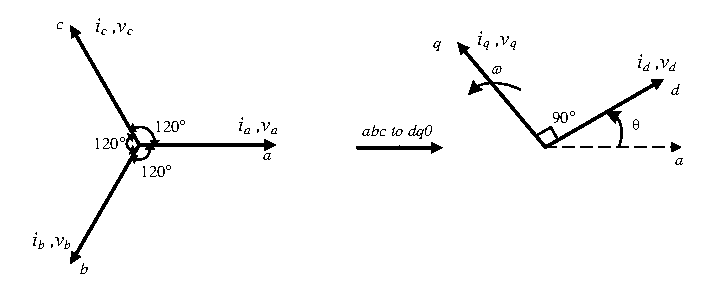
\includegraphics[scale=01]{figures/Chapter_1_2/fig2p4}
	\caption{$abc$ to $dqo$ transformation}
	\label{fig2.4}
\end{figure}

\begin{equation}
\begin{bmatrix} v_d   \\ v_q   \\ v_0 
 \end{bmatrix} or \begin{bmatrix} i_d   \\ i_q   \\ i_0 
 \end{bmatrix} = \sqrt{\frac{2}{3}}\begin{bmatrix} cos \:\theta & cos \:(\theta -2 \pi/3) & cos\: (\theta + 2 \pi/3) \\ - sin \:\theta & - sin \:(\theta -2 \pi/3) & - sin \:(\theta + 2 \pi/3) \\ \frac{1}{\sqrt{2}} & \frac{1}{\sqrt{2}} & \frac{1}{\sqrt{2}}
\end{bmatrix} \begin{bmatrix} v_a \\
 v_b  \\ v_c
\end{bmatrix} or \begin{bmatrix} i_a \\
 i_b  \\ i_c
\end{bmatrix} \\
\label{eqn2.36}
\end{equation}

The output signals of the $dq$ transformation are dependent on the performance of the phase-locked loop (PLL). The PLL circuit determines the rotation speed ($\omega$ in rad/sec) of the rotating reference frame, where $\theta$ is the angle between the $a$ and $q$ axes for the $q$-axis alignment or the angle between the $a$ and $d$ axes for the $d$-axis alignment. Depending on the presence of fundamental, harmonic, and negative sequence components in voltages and currents, the $dq$ components may have different frequencies. Analyzing these $dq$ components and applying appropriate filtering techniques can facilitate the generation of current and voltage references needed for control purposes. The $dq$ components typically comprise DC and AC components, as described below.
 \begin{equation}
 \begin{split}
 i_{Ld} =\bar{i}_{Ld} + \tilde{i}_{Ld}\\
   i_{Lq} =\bar{i}_{Lq} + \tilde{i}_{Lq}
   \end{split}
\label{eqn2.37}
\end{equation}

The DC components $\bar{i}_{Ld}$ and $\bar{i}_{Lq}$ represent the fundamental positive sequence load currents, while the AC components $\tilde{i}_{Ld}$ and $\tilde{i}_{Lq}$ correspond to the load current harmonics. The component $\bar{i}_{Lq}$ corresponds to the reactive power drawn by the load. The reference values for the compensator can be obtained as follows.
 \begin{equation}
\begin{split}
 i^*_{fd} &=- \tilde{i}_{Ld}\\
   i^*_{fq}&=-\bar{i}_{Lq} - \tilde{i}_{Lq} \\
   i^*_{f0}&=-i_{L0}
 \end{split}
\label{eqn2.38}
\end{equation}
The shunt active filter references in $abc$ reference frame are obtained as follows.
\begin{equation}
\begin{bmatrix} i^*_{fa} \\  i^*_{fb} \\   i^*_{fc}
 \end{bmatrix}=  \sqrt{\frac{2}{3}}\begin{bmatrix} cos \:\theta & - sin \:\theta & \frac{1}{\sqrt{2}} \\cos \:(\theta -2 \pi/3) & - sin \:(\theta -2 \pi/3) & \frac{1}{\sqrt{2}} \\ cos \:(\theta + 2 \pi/3) & - sin \:(\theta + 2 \pi/3) & \frac{1}{\sqrt{2}}
\end{bmatrix} \begin{bmatrix}  i^*_{fd} \\ i^*_{fq} \\  i^*_{f0}
\end{bmatrix} 
\label{eqn2.39}
\end{equation}
When the supply voltages are unbalanced or distorted, the accuracy of the transformation angle ($\theta$) obtained from the PLL may be compromised. As a result, the performance of the $dq$ transformation approach can be adversely affected in such situations. Moreover, this method involves complex transformations, and its implementation in digital signal processors (DSP) can be challenging \cite{marques1998comparison,cardenas2003comparative}."
\vspace*{-.75cm}
\subsubsection{Instantaneous Symmetrical Components Theory \cite{ghosh1998new,847283,ghosh2000use, Mahesh_Mishra}}
\vspace*{-.5cm}
"The theory of instantaneous symmetrical components is applicable for load balancing, harmonic suppression, and power factor correction. The control algorithm based on the instantaneous symmetrical component theory can partially or fully compensate for any type of load unbalance and harmonics. It achieves this by employing high-bandwidth current sources to track the filter reference currents. This control algorithm has been developed and elucidated in this section. According to the symmetrical component theory, any three-phase instantaneous quantities can be expressed in terms of positive, negative, and zero sequences using the equation provided below \cite{lyon1954transient}.
 \begin{equation}
\begin{bmatrix} i^0_{sa} \\  i^+_{sa} \\   i^-_{sa}
 \end{bmatrix}=  \frac{1}{3}\begin{bmatrix} 1 & 1 & 1 \\1 & a & a^2 \\ 1 & a^2 & a
\end{bmatrix} \begin{bmatrix}  i_{sa} \\ i_{sb} \\  i_{sc}
\end{bmatrix} ;\
 \begin{bmatrix} v^0_{sa} \\  v^+_{sa} \\   v^-_{sa}
 \end{bmatrix}=  \frac{1}{3}\begin{bmatrix} 1 & 1 & 1 \\1 & a & a^2 \\ 1 & a^2 & a
\end{bmatrix} \begin{bmatrix}  v_{sa} \\ v_{sb} \\  v_{sc}
\end{bmatrix}
\label{eqn2.40}
\end{equation}
In (\ref{eqn2.40}), the symbols $+$, $-$ and $0$ represent the positive, negative and zero sequence components, respectively. The complex operator `$a$' is equal to $e^{j120^0}$. It should be noted that the instantaneous positive sequence ($i^+_{sa}$) and negative sequence ($i^-_{sa}$) components are complex conjugates of each other, while the zero sequence component ($i^0_{sa}$) is a real quantity that equals zero when the currents are balanced. Similar to the $pq$ theory, it is assumed that the supply voltages are balanced. 

The objective of a three-phase four-wire system is to ensure the provision of a balanced supply current in which the zero sequence component is zero. Consequently, the following condition is obtained.
\begin{equation}
i_{sa}+i_{sb}+i_{sc}=0
\label{eqn2.41}
\end{equation}
The angle between the positive sequence components of the source current ($i^+_{sa}$) and the source voltage ($v^+_{sa}$) is equal to the power factor angle ($\varphi^+$) between the balanced source currents and voltages. In the control algorithm, this power factor angle can be explicitly set to any desired value. However, in the previously described $pq$ theory, the power factor angle is not directly expressed. Assuming that the phase of $i^+_{sa}$ lags behind that of $v^+_{sa}$ by an angle ($\varphi^+$), we obtain the following relationship.
\begin{equation}
\angle {\left\{v_{sa}+av_{sb}+a^2v_{sc}\right\}} = \angle {\left\{i_{sa}+ai_{sb}+a^2i_{sc}\right\}}+ \varphi^+
\label{eqn2.42}
\end{equation}
After substituting the values for $a$ and $a^2$ into (\ref{eqn2.42}), it expands to the following expression:
\begin{equation}
\angle \left\{ (v_{sa}-\frac{1}{2}v_{sb}- \frac{1}{2}v_{sc}) - j\frac{\sqrt{3}}{2} (v_{sb}-v_{sc}) \right\} = \angle \left\{ (i_{sa}-\frac{1}{2}i_{sb}- \frac{1}{2}i_{sc}) - j\frac{\sqrt{3}}{2} (i_{sb}-i_{sc}) \right\}+ \varphi^+.
\label{eqn2.43}
\end{equation}
By equating the angles in the above equation, the following expression can be written.
\begin{equation}
tan^{-1}(K_1/K_2) = tan^{-1}(K_3/K_4)+\varphi^+
\label{eqn2.44}
\end{equation}
Where,
\begin{align*}
K_1 &= \frac{\sqrt{3}}{2} (v_{sb}-v_{sc})& 
 K_2 & = \Big(v_{sa}-\frac{1}{2}v_{sb}- \frac{1}{2}v_{sc}\Big) \\
  K_3 & = \frac{\sqrt{3}}{2} (i_{sb}-i_{sc}) & 
  K_4 &= \Big(i_{sa}-\frac{1}{2}i_{sb}- \frac{1}{2}i_{sc}\Big).
\label{eqn2.44a}
\end{align*}
By taking the tangent of both sides of (\ref{eqn2.44}), the following is obtained.
\begin{equation}
\frac{K_1}{K_2} = tan\left[tan ^{-1}(K_3/K_4) + \varphi^+ \right] = \frac{K_3/K_4 + tan \: \varphi^+ }{1- (K_3/K_4)tan \: \varphi^+}
\label{eqn2.45}
\end{equation}
By substituting the values of $K_1$, $K_2$, $K_3$, and $K_4$ into the above equation, the following is obtained.
\begin{equation}
\begin{split}
(v_{sb}-v_{sc}-3\gamma (v_{sa}-v_0))i_{sa}+(v_{sc}-v_{sa}-3\gamma (v_{sb}-v_0))i_{sb}+ \\
(v_{sa}-v_{sb}-3\gamma (v_{sc}-v_0))i_{sc} = 0
\end{split}
\label{eqn2.46}
\end{equation}
Where $\gamma \equiv tan \varphi^+/\sqrt{3}$. For a unity power factor, $\varphi^+$ = 0, hence $\gamma = 0$. It is well known that in a balanced three-phase circuit, the instantaneous power remains constant, while in an unbalanced circuit, it exhibits a double-frequency component in addition to the DC or mean value. The presence of harmonics introduces higher-frequency oscillating components in the instantaneous power. The objective of the compensator is to supply the oscillating component of the instantaneous load power, while the source provides the average value of the load power, $P_{lavg}$. Therefore, the following expression is obtained.
\begin{equation}
v_{sa}i_{sa}+v_{sb}i_{sb}+v_{sc}i_{sc}=P_{lavg}
\label{eqn2.47}
\end{equation}
Since the harmonic component in the load does not require any real power, the source only needs to supply the real power required by the load. The average load power can be calculated using a moving average filter. By combining equations (\ref{eqn2.41}), (\ref{eqn2.46}), and (\ref{eqn2.47}), we obtain the reference source currents as follows:

\begin{equation}
\begin{bmatrix} i^*_{sa} \\  i^*_{sb} \\   i^*_{sc}
 \end{bmatrix}= M^{-1} 
\begin{bmatrix} 0 \\ 0 \\  P_{lavg}
\end{bmatrix}.
\label{eqn2.48}
\end{equation}
Where,
\begin{equation*}
M = {\begin{bmatrix} 1 & 1 & 1 \\ (v_{sb}-v_{sc}-3\gamma (v_{sa}-v_0)) & (v_{sc}-v_{sa}-3\gamma (v_{sb}-v_0)) & (v_{sa}-v_{sb}-3\gamma( v_{sc}-v_0)) \\ v_{sa} & v_{sb} & v_{sc}
\end{bmatrix}}.
\label{eqn2.48a}
\end{equation*}
The reference compensator currents are given as,
\begin{equation}
\begin{split}
i^{*}_{fa} =  i_{la} - i^{*}_{sa} = i_{la}- \frac{(v_{sa}-v_{0})+\gamma(v_{sb}-v_{sc})}{\Delta_1}(P_{lavg}), \\
i^{*}_{fb} =  i_{lb} - i^{*}_{sb} = i_{lb}- \frac{(v_{sb}-v_{0})+\gamma(v_{sc}-v_{sa})}{\Delta_1}(P_{lavg}), \\
i^{*}_{fc} =  i_{lc} - i^{*}_{sc} = i_{lc}- \frac{(v_{sc}-v_{0})+\gamma(v_{sa}-v_{sb})}{\Delta_1}(P_{lavg}).
\end{split}
\label{eqn2.49}
\end{equation}
Where,
\begin{equation}
\Delta_1 = \left[\sum_{j=a,b,c} v^{2}_{sj}\right] - 3 v^2_0, \ v_0 = \frac{1}{3}\sum_{k = a,b,c} v_{sk}, \ \gamma = tan \: \varphi/\sqrt{3}.
\label{eqn2.50}
\end{equation}
When incorporating the inverter power loss $P_{loss}$ into (\ref{eqn2.49}), the modified reference currents of the compensator become:
\begin{equation}
\begin{split}
i^{*}_{fa} =  i_{la} - i^{*}_{sa} = i_{la}- \frac{(v_{sa}-v_0)+\gamma(v_{sb}-v_{sc})}{\Delta_1}(P_{lavg}+P_{loss}), \\
i^{*}_{fb} =  i_{lb} - i^{*}_{sb} = i_{lb}- \frac{(v_{sb}-v_0)+\gamma(v_{sc}-v_{sa})}{\Delta_1}(P_{lavg}+P_{loss}), \\
i^{*}_{fc} =  i_{lc} - i^{*}_{sc} = i_{lc}- \frac{(v_{sc}-v_0)+\gamma(v_{sa}-v_{sb})}{\Delta_1}(P_{lavg}+P_{loss}).
\end{split}
\label{eqn2.51}
\end{equation}
In the described system, the term $P_{lavg}$ represents the average power required by the load, which is obtained using a simple moving average filter over a half cycle. The oscillating part of the real power has a frequency that is double the system frequency. The term $P_{loss}$ is obtained from a proportional-integral (PI) controller. The error between the DC voltage reference and the actual DC voltage is processed through the PI controller to obtain $P_{loss}$. This control mechanism helps to regulate the DC-link voltage by adjusting the small amount of real power absorbed by the shunt inverter. The reference current of the shunt active filter contains not only reactive and harmonic components but also some amount of active current as compensating current. This active compensating current flows through the shunt active filter and helps to regulate the DC capacitor voltage \cite{ghosh2000use}. The shunt active filter draws this active current from the AC source, to recharge the DC capacitor. It should be noted that when the source voltages are balanced, the zero sequence voltage $v_0$ is equal to zero in the above equations.

When the source voltages used for generating the shunt filter current references are unbalanced and distorted, it can lead to erroneous compensation using the conventional shunt algorithm \cite{4519806}. To overcome this limitation, an improved approach is proposed where the fundamental positive sequence voltages $v^{+}_{sa1}(t)$, $v^{+}_{sb1}(t)$ and $v^{+}_{sc1}(t)$ of the PCC voltages are extracted. These extracted voltages are then used in the shunt algorithm to generate the reference compensator currents, as given below.
\begin{equation}
\begin{split}
i^{*}_{fa} =  i_{la} - i^{*}_{sa} = i_{la}- \frac{v^{+}_{sa1}+\gamma^+(v^{+}_{sb1}-v^{+}_{sc1})}{\Delta^{+}_1}(P_{lavg}+P_{loss})\\
i^{*}_{fb} =  i_{lb} - i^{*}_{sb} = i_{lb}- \frac{v^{+}_{sb1}+\gamma^+(v^{+}_{sc1}-v^{+}_{sa1})}{\Delta^{+}_1}(P_{lavg}+P_{loss})\\
i^{*}_{fc} =  i_{lc} - i^{*}_{sc} = i_{lc}- \frac{v^{+}_{sc1}+\gamma^+(v^{+}_{sa1}-v^{+}_{sb1})}{\Delta^{+}_1}(P_{lavg}+P_{loss})
\end{split}
\label{eqn2.52}
\end{equation}
Where, 
\begin{equation}
\begin{split}
\Delta^+_1 = \sum_{j=a,b,c} (v^{+}_{sj1})^2; ~~ \gamma^+ = tan \: \varphi^+/\sqrt{3}.
\end{split}
\label{eqn2.53}
\end{equation}
Out of various theories discussed above, the instantaneous symmetrical component theory with the extraction of fundamental positive sequence components offers a simple and clear formulation for power system control. It eliminates ambiguity in definitions of various power terms and provides flexibility in handling various load and voltage conditions. Its compactness makes it suitable for implementation in digital signal processors, enabling real-time and effective compensation \cite{4519806,mahesh2010dsp}."

\subsection {Generation of Reference Quantities for DVR}
The voltage compensation method can be chosen based on factors such as the dynamic voltage restorer's (DVR) power rating, load characteristics, operating conditions, the load's susceptibility to phase angle jumps, and fault types \cite{DVR}. There are three main voltage injection/compensation strategies that can be employed.  
\vspace*{-.5cm}
\subsubsection{Pre-Sag Compensation} \vspace*{-.5cm}
"In order to keep the load voltage at the pre-sag level, the pre-sag compensation method continually monitors the supply voltage and generates a compensation voltage. It is particularly suitable for sensitive loads that are adversely affected by sudden changes in phase angle. However, supplying both active and reactive powers from the VSI is required for this technique, which also demands for a higher-rated DVR. Due to the fact that this scheme uses active power from the VSI, DVR requires a large energy storage capacity. 

The per phase phasor diagram of the pre-sag compensation shows that the pre-sag and post-sag voltages are at the same position, i.e., $V_{pre-sag} = V_{post-sag}$. In the phasor diagram, the change in phase angle of the grid terminal voltage $V_{tsag}$ is denoted as $\theta$, the load current is denoted as $I_{l}$ and the load power factor angle is denoted as $\phi$. The phasor angles are defined with respect to load current.  In order to adjust the load voltage to its pre-sag value as part of the compensation, a voltage of $V_{dvr} = V_{inj}$ is injected. Phase-locked loops (PLLs) must be used with this technique in order to synchronise with the load voltages. The magnitude and phase angle ($\alpha$) of the DVR injection voltage, as well as the active and reactive power associated with load voltage compensation, are calculated based on the phase jump of the grid voltage and sag depth. The equations for these calculations are given in \eqref{2.pre_sag11} - \eqref{2.pre_sag14}."
\vspace*{-1.2cm}
\begin{figure}[h!]
	\centering
   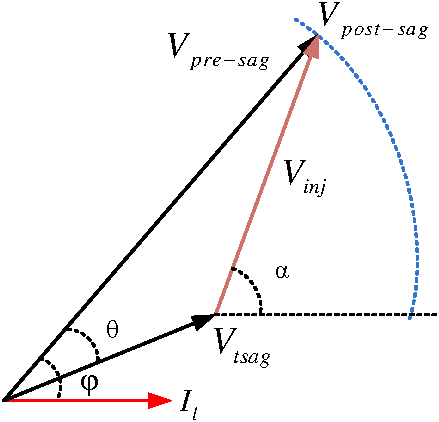
\includegraphics[scale=0.85]{figures/Chapter_1_2/c2_pre_sag}
   \caption{Per phase phasor diagram for pre-sag compensation \cite{ManikPradhan}}
   \label{2.pre_sag}
\end{figure}
\vspace*{-1.5cm}
\begin{eqnarray}
\label{2.pre_sag10}
\left|V_{dvr}\right| &=& \sqrt{V^{2}_{pre-sag}-2V^{}_{pre-sag}V^{}_{tsag}\cos\theta+V^{2}_{tsag}} \label{2.pre_sag11}\\
\angle V_{dvr} = \alpha &=&\tan^{-1}\bigg(\frac{V_{pre-sag}\sin\phi - V_{tsag}\sin (\phi - \theta)}{V_{pre-sag} \cos \phi -V_{tsag}\cos (\phi - \theta) } \label{2.pre_sag12}\bigg)\\
 P_{dvr} &=& \left|V_{dvr}\right| I_{l}\cos \alpha\label{2.pre_sag13}\\
 Q_{dvr} &=& \left|V_{dvr}\right| I_{l}\sin \alpha\label{2.pre_sag14}
\end{eqnarray} 

%%%%%%%%%%%%%%%%%%%%%%%%%%%%%%%%%%%
\subsubsection{In-Phase Compensation}
"The supply voltage and the injected voltage are in phase with one another when using the in-phase compensation method. This method aims to reduce the required injection voltage, which allows for a lower voltage rating of the storage unit or DC-link bus. However, this method has to account for active power injection. It is important to note that the in-phase compensation method only mitigates the load voltage magnitude but not the phase jump. Therefore, it is not appropriate for loads that are sensitive to phase jumps. The phasor diagram in Fig.\,\ref{2.inphase_sag} can be used to determine the magnitude of the DVR injection voltage as well as the active and reactive powers related to compensation of load voltages. The specific calculations are as follows:"
\begin{figure}[h!]
	\centering
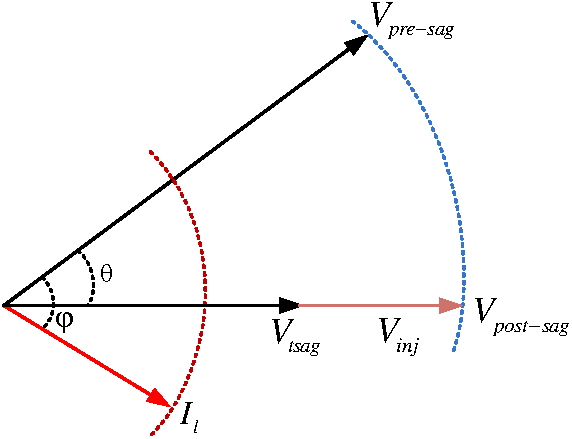
\includegraphics[scale=0.85]{figures/Chapter_1_2/c2_in_phase}
   \caption{Per phase phasor diagram for in-phase compensation \cite{ManikPradhan}}
   \label{2.inphase_sag}
\end{figure}
\begin{eqnarray}
\label{2.in_phase}
\left|V_{dvr}\right| &=& \left|V_{pre-sag}\right|-\left|V_{tsag}\right|,\\
 P_{dvr} &=& \left|V_{dvr}\right| I_{l}\cos(\phi-\theta),\\
 Q_{dvr} &=& \left|V_{dvr}\right| I_{l}\sin(\phi-\theta).
\end{eqnarray}

%%%%%%%%%%%%%%%%%%%%%%%%%%%%%%%%%%%%%%%%%%%%%%%%%%%%%% 
\vspace{-1em}
\subsubsection{Energy Optimized Compensation}
\vspace{-1em}
"The energy optimized compensation technique is employed to minimize the active power requirement of the DVR circuit. In this method, the DVR is controlled to ensure that the compensation voltages are perpendicular to the load currents, resulting in supply of zero active power by the DVR. The main objective is to absorb as much active power as possible from the grid during voltage sag, reducing the reliance on the DVR for active power compensation. While this technique minimizes the energy requirement for load voltage restoration, it does not address the phase jump that occurs during sag events. Furthermore, there is a limitation on the minimum sag depth that can be compensated without active power supply. If the grid terminal voltage drops below a certain threshold, the compensation technique will require active power supply to restore the load voltage.
\vspace*{-0.5cm}
\begin{figure}[h!]
	\centering
    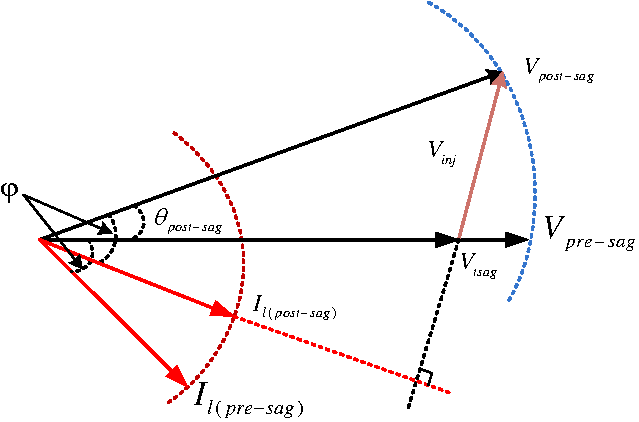
\includegraphics[scale=0.9]{figures/Chapter_1_2/c2_energy_optimize}
    \caption{Per phase phasor diagram for energy optimized load voltage compensation}
    \label{2.energy_optimized}
\end{figure} \vspace*{-0.5cm}

The magnitude of the DVR injection voltage, as well as the active and reactive powers related to the compensation of load voltages, can be calculated from the phasor diagram illustrated in Fig. \ref{2.energy_optimized}. The specific calculations are as follows:"
\begin{eqnarray}
\label{2.Energy_optimized}
\left|V_{dvr}\right| &=& \sqrt{V^{2}_{pre-sag}-2V^{}_{pre-sag}V^{}_{tsag}\cos\theta_{post-sag}+V^{2}_{tsag}} \label{2.EO11},\\
\angle V_{dvr} = \alpha &=&90^{\circ}, \label{2.EO12}
\end{eqnarray}
\begin{eqnarray}
P_{dvr} &=& 0, \label{2.EO13}\\
Q_{dvr} &=& \left|V_{dvr}\right| I_{l}\label{2.EO14}.
\end{eqnarray}
%%%%%%%%%%%%%%%%%%%%%%%%%%%%%%%%%%%%%%%%%%%

\subsection {Switching Control Techniques}

In Section \ref{2.DOC_UPQC}, various drawbacks were identified for the shunt and series control circuits that were based on linear controllers. These limitations sparked the exploration of alternative control techniques. This section aims to review the most commonly used control methods that have been developed for DSTATCOM, DVR, and conventional UPQC. 
\vspace*{-1.5cm}
\subsubsection{A. Hysteresis Control} \vspace*{-0.5cm}
Hysteresis control is a non-linear control technique that aims to make a measured signal follow its reference by using a non-linear feedback loop. This is achieved by adding a defined error of the measured signal to its reference waveform, creating upper and lower boundaries, also known as a hysteresis band. The switching actions of a converter keep the measured signal within this band \cite{605621}. Hysteresis control can be designed in different reference frames and can control current as well as voltage \cite{5951759,4510107, 4766427}.

The key benefits of hysteresis control over linear controllers include its ease of implementation, minimal tracking errors, robustness, independence from changes in load parameters, and good dynamics. However, there are some drawbacks. One is that in systems without a neutral connection, the instantaneous error of the measured signal can reach double due to the interaction between three phases \cite{720325}, and hence the three phases must be decoupled. Another drawback is that the hysteresis control produces varying switching frequency during the fundamental period, which can cause an increase in switching losses and difficulty in designing input filters.

\subsubsection{B. Constant Switching Frequency Hysteresis Controllers} \vspace*{-0.5cm}
Several design solutions were developed to overcome the main drawback of variable switching frequency inherent in hysteresis control methods. Although the functional principle of hysteresis controllers with constant switching frequency is typically the same as for conventional hysteresis techniques, the switching frequency is fixed. The first solution is a ramp controller without hysteresis \cite{4766477}, where the measured signal is compared with a modulated reference created by adding a fixed amplitude and frequency triangular carrier. Implementation of three $120^{\circ}$ phase-shifted triangular carriers is also possible \cite{605621}. However, this method generates errors in amplitude and phase of the measured signal \cite{605621}, and experiences over-crossing and under-crossing effects \cite{4766477}. The second solution is the addition of hysteresis to the ramp controller, which eliminates problems with measured signal errors and requires lower carrier frequency for overcoming crossing effects \cite{4766477}. In systems without a neutral connection, these techniques significantly degrade in performance, particularly if a DC-offset is required, as in the case of the nine-switch UPQC. As a result, these control techniques are unsuitable for replacing linear controllers. Finally, an adaptive hysteresis-band or a variable-band hysteresis controller is another solution for providing constant switching frequency, which changes the hysteresis bandwidth to provide an optimal switching frequency that remains nearly constant \cite{103436}. Although the simplicity of this hysteresis method is lost in comparison to the conventional hysteresis controller, it still provides all other advantages. This control method was implemented as a fuzzy-logic controller in the conventional UPQC to control its current and voltage \cite{4758382}, and its applicability for controlling current was demonstrated in systems without a neutral connection \cite{6199990}.
\vspace*{-0.8cm}
\subsubsection{C. Sliding Mode Control} \vspace*{-0.5cm}
Several control techniques were proposed based on the sliding mode concept, which are designed to control both current and voltage. These controllers include sliding mode control (SMC) \cite{1489536}, sliding mode pulse width modulation (SMPWM) \cite{4455458}, and hysteresis-modulation sliding mode pulse width modulation (HM-SMPWM) \cite{6563653}, all of which are designed in the $abc$ natural frame.

One of the main advantages of the sliding mode concept is its ability to provide a coherent mathematical model for decoupling interactive three-phase signals of power systems without a neutral connection. This model was proposed for controlling current in the three-phase system without a neutral connection \cite{4455458}. Another study proposed the use of the sliding mode concept to control two sets of three-phase currents of the nine-switch converter \cite{6563653}. The SMC controller proposed in \cite{1489536} was based on the SMC theory for controlling voltage in the 3P3W system. However, it did not apply the decoupling technique based on the sliding mode concept. Instead, it connected the DC-link mid-point to the neutral point of star-connected series transformers, which nullified the interaction between three-phase voltages and the use of DC-offsets/neutral-point voltages. Consequently, this control method is unsuitable for providing proper operation of the nine-switch UPQC.

\section{SUMMARY} 
This chapter provides an overview of the conventional unified power quality conditioner (UPQC), including the operation of the dual-output converter and its advantages and limitations compared to the back-to-back topology. It also discusses the previously designed nine-switch converter based UPQC. The performance of the nine-switch UPQC depends greatly on the accurate selection of its operation modes under different working conditions, as well as the control methods used for the shunt and series terminals.

The chapter examines the control methods that have already been applied in the nine-switch UPQC, which utilize linear controllers and have shown satisfactory results. However, these methods have certain drawbacks that have prompted the search for alternative solutions. Non-linear control methods have been presented for controlling two sets of three-phase currents in the nine-switch converter. However, no potential replacement has been found for the series terminal controller. Additionally, the generation of reference quantities requires an accurate estimation of the grid voltage phase angle. Therefore, Chapter \ref{3.Chap:PLL} discusses the performance comparison of advanced phase-locked loops (PLLs). Furthermore, Chapter \ref{4.Chap:DSTATCOM} presents the proposed sliding mode control for the four-leg distribution static synchronous compensator (DSTATCOM), Chapter \ref{5.Chap:DVR} focuses on the four-leg dynamic voltage restorer (DVR), and Chapter \ref{6.Chap:DOCUPQC} covers the four-leg dual-output converter based UPQC.